%archivo del Ap�ndice

\chapter{Ap�ndices} \label{apex}

\section{Ap�ndice A: Tutorial Uso Del Programa De Corte} \label{apex1}

En este ap�ndice se describe el uso del programa de cortado desarrollado.

En la figura \ref{GUI1} se muestra la interfaz gr�fica.

\begin{figure}[!htb]
        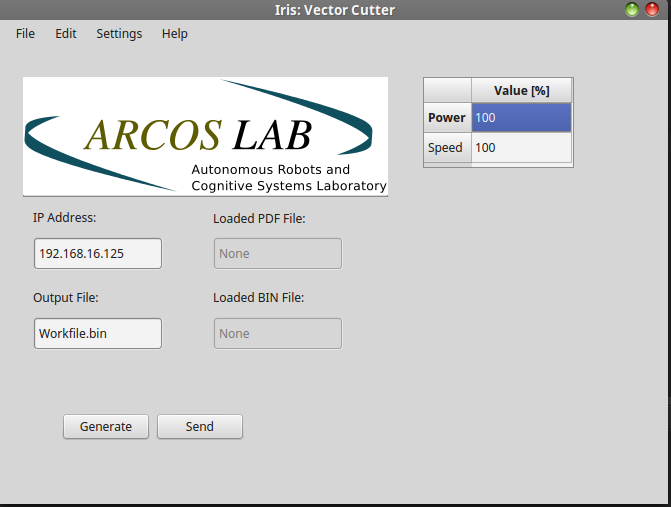
\includegraphics[width=0.5\linewidth]{./Figuras/GUI}
        \caption{GUI del software de cortado.} 
        \label{GUI1}
\end{figure}

El primer paso para realizar el corte es cargar el archivo PDF, para ello se selecciona la opci�n Load PDF en el menu FILE. Esto nos muestra una ventana de dialogo donde podemos seleccionar el archivo PDF deseado como se observa en la figura \ref{GUI2}.

\begin{figure}[!htb]
        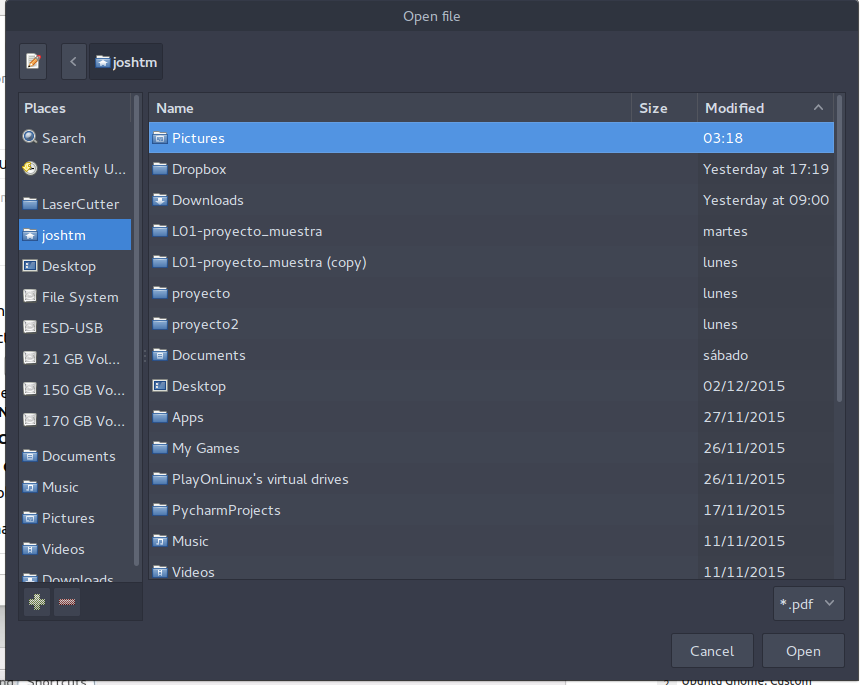
\includegraphics[width=0.5\linewidth]{./Figuras/GUI2}
        \caption{Dialogo de selecci�n de archivo.} 
        \label{GUI2}
\end{figure}

Una vez seleccionado el archivo PDF, su nombre aparece bajo el cuadro Loaded PDF lo cual nos asegura que el archivo fue cargado con �xito.

El siguiente paso es seleccionar un nombre para el archivo de salida, para ello se escribe el nombre deseado y su extensi�n en el cuadro Output File como se observa en la figura \ref{GUI3}. Por default el nombre del archivo es Workfile.bin.

\begin{figure}[!htb]
        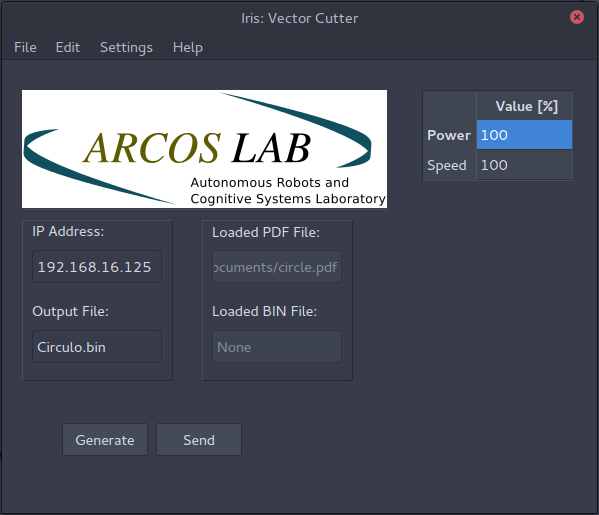
\includegraphics[width=0.5\linewidth]{./Figuras/GUI3}
        \caption{Selecci�n del archivo de salida.} 
        \label{GUI3}
\end{figure}


El siguiente paso es seleccionar una potencia de salida, para ello se cambia el valor de Power en el cuadro localizado en la esquina superior derecha. Una vez hecho esto, se procede a darle click en el bot�n Generate. Al final la creaci�n del archivo de corte aparecer� una ventana con un preview del corte a realizar como se muestra en la figura \ref{GUI4}. 

\begin{figure}[!htb]
        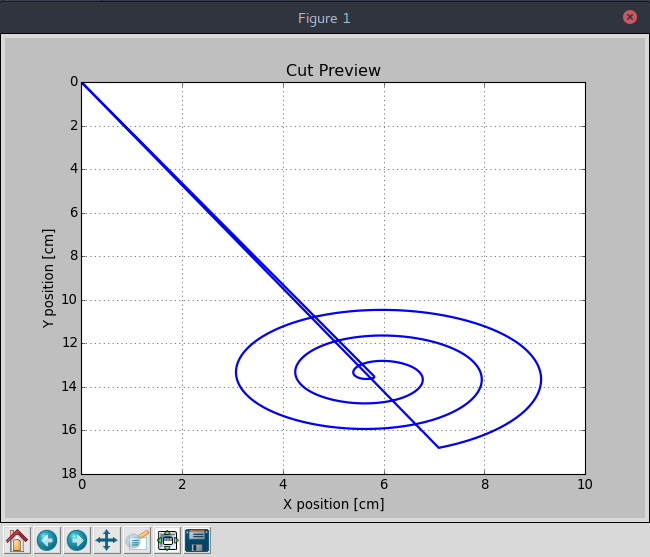
\includegraphics[width=0.5\linewidth]{./Figuras/GUI4}
        \caption{Ventana que contiene un vistazo preliminar del corte.} 
        \label{GUI4}
\end{figure}

Al cerrar esta ventana aparecer� el nombre del archivo de corte cargado en el cuadro Loaded Binary File como se observa en la figura \ref{GUI5}. Si se est� satisfecho con el preview del corte, el siguiente paso es enviarlo a la cortadora l�ser para realizar el corte. 

\begin{figure}[!htb]
        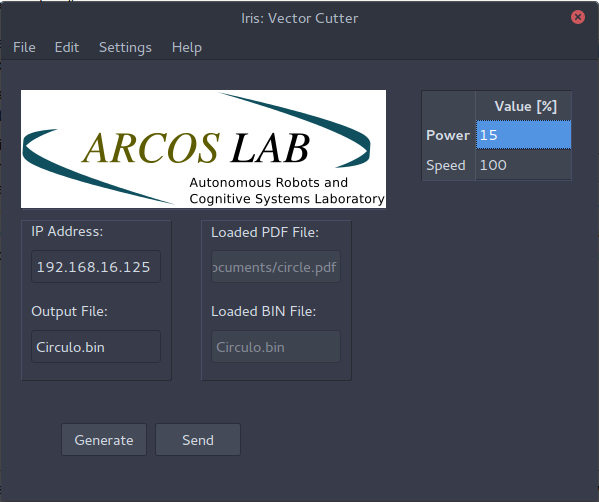
\includegraphics[width=0.5\linewidth]{./Figuras/GUI5}
        \caption{Ventana que contiene un vistazo preliminar del corte.} 
        \label{GUI5}
\end{figure}

Para utilizar la cortadora l�ser es necesario seguir los pasos de seguridad planteados en: \url{https://wiki.arcoslab.eie.ucr.ac.cr/doku.php/internal:cortadora_laser}.

Una vez encendida, la cortadora l�ser indicara su direcci�n IP asignada, este valor deber� ser introducido en el cuadro IP Address. 

El paso final es hacer click en el bot�n Send, si no ocurre ning�n inconveniente, la cortadora comenzar� a realizar el trabajo de corte.  

\clearpage
\newpage

\section{Ap�ndice B: C�digo Completo de la GUI} \label{apex2}

\begin{lstlisting}[language=Python, caption= C�digo Completo de la GUI .]

from PyQt4 import QtCore, QtGui
import os
import VectorCut
import socket

try:
    _fromUtf8 = QtCore.QString.fromUtf8
except AttributeError:
    def _fromUtf8(s):
        return s

try:
    _encoding = QtGui.QApplication.UnicodeUTF8
    def _translate(context, text, disambig):
        return QtGui.QApplication.translate(context, text, disambig, _encoding)
except AttributeError:
    def _translate(context, text, disambig):
        return QtGui.QApplication.translate(context, text, disambig)


class Ui_MainWindow(object):


    def setupUi(self, MainWindow):
        MainWindow.setObjectName(_fromUtf8("MainWindow"))
        MainWindow.resize(661, 480)
        
        self.centralwidget = QtGui.QWidget(MainWindow)
        self.centralwidget.setObjectName(_fromUtf8("centralwidget"))

        # ScrollArea instance
        self.scrollArea = QtGui.QScrollArea(self.centralwidget)

        # ScrollArea image
        self.Output_label = QtGui.QLabel(self.scrollArea)
        self.Output_label.setObjectName(_fromUtf8("Output_label"))
        self.image = QtGui.QPixmap("arcoslabrev3a.png")

        # ScrollArea properties
        self.scrollArea.setGeometry(QtCore.QRect(20, 30, 365, 120))
        self.scrollArea.setWidgetResizable(True)
        self.scrollArea.setObjectName(_fromUtf8("scrollArea"))
        self.scrollAreaWidgetContents = QtGui.QWidget(self.Output_label)
        self.scrollAreaWidgetContents.setGeometry(QtCore.QRect(0, 0, 259, 269))
        self.scrollAreaWidgetContents.setObjectName(_fromUtf8("scrollAreaWidgetContents"))
        self.scrollArea.setWidget(self.scrollAreaWidgetContents)
        # self.scrollArea.setHorizontalScrollBarPolicy(QtCore.Qt.ScrollBarAlwaysOn)
        # self.scrollArea.setVerticalScrollBarPolicy(QtCore.Qt.ScrollBarAlwaysOn)

        # table, takes the config option from the user
        self.tableWidget = QtGui.QTableWidget(self.centralwidget)
        self.tableWidget.setGeometry(QtCore.QRect(420, 30, 151, 91))
        self.tableWidget.setObjectName(_fromUtf8("tableWidget"))
        self.tableWidget.setColumnCount(1)
        self.tableWidget.setRowCount(2)
        item = QtGui.QTableWidgetItem()
        self.tableWidget.setVerticalHeaderItem(0, item)
        item = QtGui.QTableWidgetItem()
        self.tableWidget.setVerticalHeaderItem(1, item)
        item = QtGui.QTableWidgetItem()
        self.tableWidget.setHorizontalHeaderItem(0, item)
        item = QtGui.QTableWidgetItem()
        self.tableWidget.setItem(0, 0, item)
        item = QtGui.QTableWidgetItem()
        self.tableWidget.setItem(1, 0, item)

        # Central frame
        self.frame = QtGui.QFrame(self.centralwidget)
        self.frame.setGeometry(QtCore.QRect(20, 160, 151, 161))
        self.frame.setFrameShape(QtGui.QFrame.StyledPanel)
        self.frame.setFrameShadow(QtGui.QFrame.Raised)
        self.frame.setObjectName(_fromUtf8("frame"))

        self.Address_lineEdit = QtGui.QLineEdit(self.frame)
        self.Address_lineEdit.setGeometry(QtCore.QRect(10, 30, 130, 33))
        self.Address_lineEdit.setObjectName(_fromUtf8("Address_lineEdit"))
        
        self.label = QtGui.QLabel(self.frame)
        self.label.setGeometry(QtCore.QRect(10, 0, 81, 21))
        self.label.setObjectName(_fromUtf8("label"))

        # TO DO: Implement a Progress Bar
        # self.progressBar = QtGui.QProgressBar(self.frame)
        # self.progressBar.setGeometry(QtCore.QRect(10, 220, 118, 23))
        # self.progressBar.setProperty("value", 0)
        # self.progressBar.setObjectName(_fromUtf8("progressBar"))

        # self.label_2 = QtGui.QLabel(self.frame)
        # self.label_2.setGeometry(QtCore.QRect(10, 200, 65, 21))
        # self.label_2.setObjectName(_fromUtf8("label_2"))
        
        self.Output_lineEdit = QtGui.QLineEdit(self.frame)
        self.Output_lineEdit.setGeometry(QtCore.QRect(10, 110, 130, 33))
        self.Output_lineEdit.setObjectName(_fromUtf8("Output_lineEdit"))
        
        self.label_3 = QtGui.QLabel(self.frame)
        self.label_3.setGeometry(QtCore.QRect(10, 80, 111, 21))
        self.label_3.setObjectName(_fromUtf8("label_3"))

        # Central frame 2
        self.frame2 = QtGui.QFrame(self.centralwidget)
        self.frame2.setGeometry(QtCore.QRect(200, 160, 151, 161))
        self.frame2.setFrameShape(QtGui.QFrame.StyledPanel)
        self.frame2.setFrameShadow(QtGui.QFrame.Raised)
        self.frame2.setObjectName(_fromUtf8("frame"))

        # Loaded BIN File label and Line edit configurations
        self.label_BinFile = QtGui.QLabel(self.frame2)
        self.label_BinFile.setGeometry(QtCore.QRect(10, 80, 111, 21))
        self.label_BinFile.setObjectName(_fromUtf8("label_BinFile"))
        self.label_BinFile.setText(_translate("MainWindow", "Loaded BIN File:", None))

        self.OutputB_lineEdit = QtGui.QLineEdit(self.frame2)
        self.OutputB_lineEdit.setGeometry(QtCore.QRect(10, 110, 130, 33))
        self.OutputB_lineEdit.setObjectName(_fromUtf8("Output_lineEdit"))
        self.OutputB_lineEdit.setText(_translate("MainWindow", "None", None))
        self.OutputB_lineEdit.setDisabled(True)

        # Loaded PDF File label and Line edit configuration
        self.label_Loaded_PDF = QtGui.QLabel(self.frame2)
        self.label_Loaded_PDF.setGeometry(QtCore.QRect (10, 1, 111, 21))
        self.label_Loaded_PDF.setObjectName(_fromUtf8("label_Loaded_PDF"))
        self.label_Loaded_PDF.setText(_translate("MainWindow", "Loaded PDF File:", None))

        self.Loaded_PDF_lineEdit = QtGui.QLineEdit(self.frame2)
        self.Loaded_PDF_lineEdit.setGeometry(QtCore.QRect(10, 30, 130, 33))
        self.Loaded_PDF_lineEdit.setObjectName(_fromUtf8("Loaded_PDF_lineEdit"))
        self.Loaded_PDF_lineEdit.setText(_translate("MainWindow", "None", None))
        self.Loaded_PDF_lineEdit.setDisabled(True)

        # Buttons Widget properties
        self.layoutWidget = QtGui.QWidget(self.centralwidget)
        self.layoutWidget.setGeometry(QtCore.QRect(50, 350, 200, 60))
        self.layoutWidget.setObjectName(_fromUtf8("layoutWidget"))
        self.horizontalLayout = QtGui.QHBoxLayout(self.layoutWidget)
        self.horizontalLayout.setObjectName(_fromUtf8("horizontalLayout"))

        # Generate Button
        self.Gen_pushButton = QtGui.QPushButton(self.layoutWidget)
        self.Gen_pushButton.setObjectName(_fromUtf8("Gen_pushButton"))
        self.horizontalLayout.addWidget(self.Gen_pushButton)

        #Send Button
        self.Send_pushButton = QtGui.QPushButton(self.layoutWidget)
        self.Send_pushButton.setObjectName(_fromUtf8("Send_pushButton"))
        self.horizontalLayout.addWidget(self.Send_pushButton)

        self.layoutWidget.raise_()
        self.scrollArea.raise_()
        self.tableWidget.raise_()
        self.frame.raise_()
        MainWindow.setCentralWidget(self.centralwidget)

        # Menu Bar Configurations
        self.menubar = QtGui.QMenuBar(MainWindow)
        self.menubar.setGeometry(QtCore.QRect(0, 0, 661, 27))
        self.menubar.setObjectName(_fromUtf8("menubar"))
        self.menuFile = QtGui.QMenu(self.menubar)
        self.menuFile.setObjectName(_fromUtf8("menuFile"))
        self.menuEdit = QtGui.QMenu(self.menubar)
        self.menuEdit.setObjectName(_fromUtf8("menuEdit"))
        self.menuHelp = QtGui.QMenu(self.menubar)
        self.menuHelp.setObjectName(_fromUtf8("menuHelp"))
        self.menuSettings = QtGui.QMenu(self.menubar)
        self.menuSettings.setObjectName(_fromUtf8("menuSettings"))
        MainWindow.setMenuBar(self.menubar)
        self.statusbar = QtGui.QStatusBar(MainWindow)
        self.statusbar.setObjectName(_fromUtf8("statusbar"))
        MainWindow.setStatusBar(self.statusbar)
        self.actionLoad_PDF = QtGui.QAction(MainWindow)
        self.actionLoad_PDF.setObjectName(_fromUtf8("actionLoad_PDF"))
        self.actionExit = QtGui.QAction(MainWindow)
        self.actionExit.setObjectName(_fromUtf8("actionExit"))
        self.actionAbout = QtGui.QAction(MainWindow)
        self.actionAbout.setObjectName(_fromUtf8("actionAbout"))

        # Menu Options
        self.menuFile.addAction(self.actionLoad_PDF)
        #self.menuFile.addAction(self.actionLoad_BIN)
        self.menuFile.addSeparator()
        self.menuFile.addAction(self.actionExit)
        self.menuHelp.addSeparator()
        self.menuHelp.addAction(self.actionAbout)
        self.menubar.addAction(self.menuFile.menuAction())
        self.menubar.addAction(self.menuEdit.menuAction())
        self.menubar.addAction(self.menuSettings.menuAction())
        self.menubar.addAction(self.menuHelp.menuAction())

        self.retranslateUi(MainWindow)

        # Message Box, General Messages send by the app.
        self.msgBox = QtGui.QMessageBox()

        # Action Handlers for menu options and buttons.
        QtCore.QObject.connect(self.actionExit, QtCore.SIGNAL(_fromUtf8("activated()")), MainWindow.close)
        QtCore.QObject.connect(self.actionLoad_PDF, QtCore.SIGNAL(_fromUtf8("activated()")), self.load_pdf)
        QtCore.QObject.connect(self.actionAbout , QtCore.SIGNAL(_fromUtf8("activated()")), self.load_pdf)
        QtCore.QObject.connect(self.Gen_pushButton, QtCore.SIGNAL(_fromUtf8("clicked()")), self.gen_bin)
        QtCore.QObject.connect(self.Send_pushButton, QtCore.SIGNAL(_fromUtf8("clicked()")), self.send_bin)
        QtCore.QMetaObject.connectSlotsByName(MainWindow)



    def retranslateUi(self, MainWindow):

        # Windows Title: Iris Vector Cutter
        MainWindow.setWindowTitle(_translate("MainWindow", "Iris: Vector Cutter", None))

        item = self.tableWidget.verticalHeaderItem(0)
        item.setText(_translate("MainWindow", "Power", None))
        item = self.tableWidget.verticalHeaderItem(1)
        item.setText(_translate("MainWindow", "Speed", None))
        item = self.tableWidget.horizontalHeaderItem(0)
        item.setText(_translate("MainWindow", "Value [%]", None))
        __sortingEnabled = self.tableWidget.isSortingEnabled()
        self.tableWidget.setSortingEnabled(False)
        item = self.tableWidget.item(0, 0)
        item.setText(_translate("MainWindow", "100", None))
        item = self.tableWidget.item(1, 0)
        item.setText(_translate("MainWindow", "1000", None))
        self.tableWidget.setSortingEnabled(__sortingEnabled)
        self.Address_lineEdit.setText(_translate("MainWindow", "192.168.16.125", None))
        self.label.setText(_translate("MainWindow", "IP Address:", None))
        # self.label_2.setText(_translate("MainWindow", "Progress", None))
        self.Output_lineEdit.setText(_translate("MainWindow", "Workfile.bin", None))
        self.label_3.setText(_translate("MainWindow", "Output File:", None))

        #Scroll Area Output
        self.Output_label.setPixmap(self.image)

        self.Gen_pushButton.setText(_translate("MainWindow", "Generate", None))
        self.Send_pushButton.setText(_translate("MainWindow", "Send", None))
        self.menuFile.setTitle(_translate("MainWindow", "File", None))
        self.menuEdit.setTitle(_translate("MainWindow", "Edit", None))
        self.menuHelp.setTitle(_translate("MainWindow", "Help", None))
        self.menuSettings.setTitle(_translate("MainWindow", "Settings", None))
        self.actionLoad_PDF.setText(_translate("MainWindow", "Load PDF", None))

        self.actionExit.setText(_translate("MainWindow", "Exit", None))
        self.actionAbout.setText(_translate("MainWindow", "About", None))

    # Error Windows Setup
    def error_windows_raise(self, title, text, error):
        print '{}'.format(error)
        self.msgBox.setWindowTitle(title)
        self.msgBox.setText(text)
        self.msgBox.setDetailedText('{}'.format(error))
        self.msgBox.exec_()

    # PDF File Loader Method
    def load_pdf(self):
        self.PDF_PATH = QtGui.QFileDialog.getOpenFileName(self.centralwidget,'Open file', os.getenv('HOME'),'*.pdf')
        self.Loaded_PDF_lineEdit.setText(self.PDF_PATH)
        print 'Loading PDF File:\n {}\n'.format(self.PDF_PATH)

    # Binary File Generating Method
    def gen_bin(self):
        try:
            laser_power = self.tableWidget.item(0, 0)
            Polygon_Generator = VectorCut.PathGenerator(self.PDF_PATH, int(laser_power.text()))
            MyPolygon = Polygon_Generator.generate()
        except AttributeError as err:
            self.error_windows_raise('AttributeError', 'Error: No PDF file has been loaded', err)
            self.load_pdf()
            # self.gen_bin()
        except IOError as err:
            self.error_windows_raise('IOError', 'The PDF has not been found, please check the file address and try loading the file again.', err)
        else:
            print'Loading PDF file...'
            output_file = self.Output_lineEdit.text()
            print 'Reading motor speed'
            motor_speed = self.tableWidget.item(1, 0)
            print motor_speed.text()
            print 'Generating Binary File...'

            executor = VectorCut.PolygonExecuter(MyPolygon, output_file, int(motor_speed.text()))
            executor.Execute()

            print 'Binary File Generated'

            # Save The Recently Created Binary Name.
            self.OutputB_lineEdit.setText(output_file)

    # Binary File Sending Method
    def send_bin(self):
        print 'Connecting With Host...'

        try:
            # Setup the variables passed by the user.
            ipAddr  = self.Address_lineEdit.displayText()
            nameBin = self.OutputB_lineEdit.displayText()
            print nameBin

            # Load the CNC program
            file2send = open(nameBin,'r')
            job = file2send.read()
            print job

        except IOError as err:
            # Throw an Error if the Bin File does'nt exist.
            self.error_windows_raise('IOError', 'No BIN file has been loaded', err)

        else:
            try:
                # Start the connections with the ip Addres ipAddr and CNC program job.
                VectorCut.send_job(ipAddr, job)
                # Catch all connection related problems and report back to the user.
            except socket.error as err:
                self.error_windows_raise('Connection Error', 'Impossible to connect with Host', err)


if __name__ == "__main__":
    import sys
    app = QtGui.QApplication(sys.argv)
    MainWindow = QtGui.QMainWindow()
    ui = Ui_MainWindow()
    ui.setupUi(MainWindow)
    MainWindow.show()
    sys.exit(app.exec_())

\end{lstlisting}

\clearpage
\newpage



\section{Ap�ndice C: Clase PreviewGenerator} \label{apex3}

Esta clase adicional es la encargada de generar una representaci�n gr�fica de los vectores.
 
\begin{lstlisting}[language=Python, caption= Clase PreviewGenerator.]
import matplotlib.pyplot as plt

class PreviewGenerator(object):
    def __init__(self, path):
        self.path = path

    def show(self):

        print ('Generating Preview ...\n')

        x = []
        y = []

        # Saves all the vectors in self.path, x contains all points in the X axis
        # y contains all points in the Y axis
        for i in range(len(self.path)):
            CurrVector = self.path[i]
            x.append((CurrVector.__StartingPoint__[0]/72.0)*2.54)
            y.append((CurrVector.__StartingPoint__[1]/72.0)*2.54)
            x.append((CurrVector.__EndingPoint__[0]/72.0)*2.54)
            y.append((CurrVector.__EndingPoint__[1]/72.0)*2.54)

        # Plot al vectors
        plt.plot(x, y, lw=2)

        # The Y axis is inverted for the laser cutter
        plt.gca().invert_yaxis()

        # Axis names
        plt.ylabel('Y position [cm]')
        plt.xlabel('X position [cm]')
        plt.title('Cut Preview')

        # Show plot
        plt.grid(True)
        plt.show()
\end{lstlisting}

\clearpage
\newpage


\section{Ap�ndice D: Libreria VectorCut} \label{apex4}

En este ap�ndice se incluye el c�digo completo de la librer�a VectorCut, esta librer�a incluye todos las definiciones y clases necesarias para la implementaci�n del programa de cortado.

\begin{lstlisting}[language=Python, caption= Librer�a Vector Cut.]


import math
import zlib
import scipy
import copy
import socket
from collections import deque
import libJob as lj

import numpy as np
from scipy.interpolate import pchip
import matplotlib.pyplot as plt

# Classes
class VectorCut(object):
    # Constructor
    def __init__(self, start=[0.0, 0.0], end=[0.0, 0.0], power=0.0):
        self.__StartingPoint__ = start
        self.__EndingPoint__ = end
        self.__LaserPower__ = power
        self.__DeltaX__ = abs((self.__EndingPoint__[0] - self.__StartingPoint__[0]))
        self.__DeltaY__ = abs((self.__EndingPoint__[1] - self.__StartingPoint__[1]))

    # Print
    def __repr__(self):
        return '< {} , {} > \n'.format(self.__StartingPoint__, self.__EndingPoint__)

    def __add__(self, other):
        """
        :param other:A second Vector Class Object
        :return: This method returns a new Vector Cut formed by the starting point of the
                 first vector, the ending point of the second and the power of the first vector
        """
        assert type(other) is VectorCut, 'Other is not a Vector Class Object: Object type received {}'.format(type(other))
        return VectorCut(self.__StartingPoint__, other.GetEnd(), self.__LaserPower__)

    # Set Vector Starting Point
    def SetStart(self, X0, Y0):
        self.__StartingPoint__[0] = X0
        self.__StartingPoint__[1] = Y0

    # Get Vector Starting Point
    def GetStart(self):
        return self.__StartingPoint__

    # Set Ending Point
    def SetEnd(self, Xf, Yf):
        self.__EndingPoint__[0] = Xf
        self.__EndingPoint__[1] = Yf

    # Get Ending Point
    def GetEnd(self):
        return self.__EndingPoint__

    # Set Laser Power
    def SetLaserPower(self, Power=0):
        self.__LaserPower__ = Power

    def GetLaserPower(self):
        return self.__LaserPower__

    def ScaleVector(self, Scale=1.0):
        self.__StartingPoint__[0] *= Scale
        self.__StartingPoint__[1] *= Scale
        self.__EndingPoint__[0] *= Scale
        self.__EndingPoint__[1] *= Scale

    def GetMagnitude(self):
        return math.sqrt(math.pow(self.__DeltaX__, 2) + math.pow(self.__DeltaY__, 2))

    def GetAngle(self):
        return math.degrees(math.atan2(self.__DeltaY__, self.__DeltaX__))

    def GetDeltaX(self):
        return self.__DeltaX__

    def GetDeltaY(self):
        return self.__DeltaY__


class PolygonCut(object):
    # Constructor
    def __init__(self):
        self.__Queue__ = deque([])

    # Print overload
    def __repr__(self):
        return "{}".format(self.__Queue__)

    # Length of the polygon, how many vectors form the polygon
    def __len__(self):
        return len(self.__Queue__)

    # Set item operator Overload
    def __setitem__(self, key, item):
        self.__Queue__[key] = item

    # Get Item Overload
    def __getitem__(self, key):
        return self.__Queue__[key]


    # Add a vector to the polygon
    def append(self, Vector):
        self.__Queue__.append(Vector)

    # Remove a Vector from the polygon
    def pop(self):
        return self.__Queue__.popleft()


class PolygonExecuter(object):
    def __init__(self, polygon, output_file, speed):
        self.__Polygon__ = polygon
        self.__OutputFile__ = output_file
        self.__speed__ = speed

    def SetPolygon(self, polygon):
        self.__Polygon__ = polygon

    def GetPolygon(self):
        return self.__Polygon__

    def Execute(self):
        commands = ''
        print self.GetPolygon()

        # Preview Of The Cut
        preview = PreviewGenerator(copy.deepcopy(self.GetPolygon()))

        for Vector in range(len(self.__Polygon__)):
            CurrVector = copy.deepcopy(self.__Polygon__.pop())
            CurrVector.ScaleVector(0.0139)
            print CurrVector
            # makes the cut commands
            cut = lj.vectorMove()
            commands += cut.makeCmds([CurrVector.GetStart(), CurrVector.GetEnd()], self.__speed__, CurrVector.GetLaserPower())

        # makes and stores the fullpacket in job
        print commands
        laser_bin = lj.jobPacket(commands)
        laser_bin.makePacket()
        job = laser_bin.getBin()

        # the job is written to a file
        with open(self.__OutputFile__, 'w') as bin:
            bin.write(job)
        bin.close()

        # Show Preview
        preview.show()


class CommandsGenerator(object):
    def __init__(self, VectorCut):
        self.Current_Vector = VectorCut
        self.Commands = ''

    def _cut_command_(self, Sign, Stp_X, Stp_Y):
        self.commands += '{}{}{}{}'.format(Sign, Stp_X, Stp_Y, self._get_power_())

    def _get_power_(self):
        PD = self.Current_Vector.GetLaserPower()
        P=int(PD*(255.0/100.0))
        return chr(P)

    def __XYInterpolation__(self):
        # current position is set to the starting position
        X0 = self.Current_Vector.Get_Start()[0]
        Y0 = self.Current_Vector.Get_Start()[1]
        Xf = self.Current_Vector.Get_End()[0]
        Yf = self.Current_Vector.Get_End()[1]

        # current position is set to the starting position
        X = X0
        Y = Y0

        # X Axis direction, if the value of DX is positive, the laser move to
        # the rigth if the value is negative the laser move to the left.

        DX = Xf - X0
        SignX = chr(0)
        SignY = chr(0)
        if DX >= 0:
            StepX = 1
            SignX = chr(1)
        else:
            StepX = -1

        # Y Axis direction, if the value of DY is positive, the laser move up
        # if the value is negative the laser down.

        DY = Yf - Y0

        if DY >= 0:
            StepY = 1
        else:
            StepY = -1
            SignY = chr(2)

        # Current funtion symbol, if FXY is greater than or equal to zero, the
        # laser must move in the X axis, else the laser move in the Y axis
        FXY = math.fabs(DX) - math.fabs(DY)

        # Main loop:
        while not ((X == Xf) and (Y == Yf)):

            if FXY >= 0:
                X += StepX
                FXY -= math.fabs(DY)
                self._cut_command_(SignX, '\x01', '\x00')

            else:
                Y += StepY
                FXY += math.fabs(DX)

                self._cut_command_(SignY, '\x00', '\x01')
            print('Current  point =  [{},{}]').format(X, Y)
            print(self.Commands)


class PostScriptInterpreter(object):
    def __init__(self, power=0.0):
        self.stack = []
        self.width = 0.0
        self.setrgbcolor = []
        self.Graphic_Matrix = []
        self.CurrentPosition = [0.0, 0.0]
        self.StartingPosition = [0.0, 0.0]
        self.Polygon = PolygonCut()
        self.__power__ = power

    def __isfloat__(self, value):
        try:
            float(value)
            return True
        except:
            return False

    def SetPolygon(self, polygon):
        self.Polygon = polygon

    def GetPolygon(self):
        return self.Polygon

    def __Gsave__(self):
        print 'Saving Graphics state'

    def __Grestore__(self):
        print 'Restoring Graphics state'
        self.Polygon.append(VectorCut(self.CurrentPosition, [0, 0], 0.0))
        self.CurrentPosition = [0, 0]
        self.StartingPosition = [0, 0]

    def __SetRgbColor__(self):
        while self.stack:
            self.setrgbcolor.append(self.stack.pop())
        print self.setrgbcolor

    def __GraphicsStateParam__(self):
        print 'Set parameters from graphics state parameter dictionary'

    def __Moveto__(self):
        YMovement= float(self.stack.pop())
        XMovement= float(self.stack.pop())
        self.Polygon.append(VectorCut(self.StartingPosition, [XMovement, YMovement], 0.0))
        self.CurrentPosition = [XMovement, YMovement]
        self.StartingPosition = [XMovement, YMovement]

    def __Lineto__(self):
        """
        This method takes 2 operands in the stack and form a point using the first operand as the
        Y coordinate and the second as the X coordinate, then its generates vector using the CurrentPosition
        as starting point and the produced point as ending point.
        :return: Adds The generated Vector to the Path
        """
        YMovement= float(self.stack.pop())
        XMovement= float(self.stack.pop())
        self.Polygon.append(VectorCut(self.CurrentPosition, [XMovement, YMovement], self.__power__))
        self.CurrentPosition = [XMovement, YMovement]

    def __ClosePath__(self):
        self.Polygon.append(VectorCut(self.CurrentPosition, self.StartingPosition, self.__power__))
        self.CurrentPosition = self.StartingPosition
#        self.Polygon.append(VectorCut(self.CurrentPosition, [0, 0], 0.0))
#        self.CurrentPosition = [0, 0]
#        self.StartingPosition = [0, 0]

    def __Square__(self):
        square_height = float(self.stack.pop())
        square_width = float(self.stack.pop())
        square_Y0 = float(self.stack.pop())
        square_X0 = float(self.stack.pop())

        Point1 = [square_X0, square_Y0]
        Point2 = [square_X0+square_width, square_Y0]
        Point3 = [square_X0+square_width, square_Y0+square_height]
        Point4 = [square_X0, square_Y0+square_height]

        self.Polygon.append(VectorCut(self.CurrentPosition, Point1))
        self.Polygon.append(VectorCut(Point1, Point2, self.__power__))
        self.Polygon.append(VectorCut(Point2, Point3, self.__power__))
        self.Polygon.append(VectorCut(Point3, Point4, self.__power__))
        self.Polygon.append(VectorCut(Point4, Point1, self.__power__))
        self.CurrentPosition = Point1

    def __Curveto__(self):

        # Starting Point
        Y0= self.CurrentPosition[1]
        X0= self.CurrentPosition[0]

        # Ending Point
        Y3= float(self.stack.pop())
        X3= float(self.stack.pop())

        # Bezier Control Points
        Y2= float(self.stack.pop())
        X2= float(self.stack.pop())
        Y1= float(self.stack.pop())
        X1= float(self.stack.pop())

        # Setup the parametrization
        number_of_points = 50
        t = scipy.linspace(0, 1, number_of_points)

        # Use the Bezier formula
        Bx = (1-t)**3*X0 + 3*(1-t)**2*t*X1 + 3*(1-t)*t**2*X2 + t**3*X3
        By = (1-t)**3*Y0 + 3*(1-t)**2*t*Y1 + 3*(1-t)*t**2*Y2 + t**3*Y3

        bpc = 0  # Bezier Point Counter

        #Bezier Vector Generator
        for point in t:
            xpos = Bx[bpc]
            ypos = By[bpc]
            CurrentPos = [xpos, ypos]
            tempVector = VectorCut(self.CurrentPosition, CurrentPos, self.__power__)


            self.Polygon.append(VectorCut(self.CurrentPosition, CurrentPos, self.__power__))
            self.CurrentPosition = CurrentPos


            #if (tempVector.GetDeltaX() == 0) and (tempVector.GetDeltaY()/72 > 0.0001):
            #    self.Polygon.append(VectorCut(self.CurrentPosition, CurrentPos, self.__power__))
            #    self.CurrentPosition = CurrentPos

            #elif (tempVector.GetDeltaY() == 0) and (tempVector.GetDeltaX()/72 > 0.0001):
            #    self.Polygon.append(VectorCut(self.CurrentPosition, CurrentPos, self.__power__))
            #    self.CurrentPosition = CurrentPos


            #elif (tempVector.GetDeltaX()/72 > 0.0001) and (tempVector.GetDeltaY()/72 > 0.0001):
            #    self.Polygon.append(VectorCut(self.CurrentPosition, CurrentPos, self.__power__))
            #    self.CurrentPosition = CurrentPos

            bpc += 1
        self.CurrentPosition = [X3, Y3]

    def __SetMitterLimit__(self):

        print 'Set Miter Limit'
        print self.stack.pop()

    def __SetDashPattern__(self):

        print 'Set Dash Pattern:'
        if self.stack.pop() == '0.0':
            print 'No Dash'

    def __Stroke__(self):

        print 'Stroking Current Path'

    def __SetLineWidth__(self):
         self.width=self.stack.pop()
         print 'Set line Width'
         print self.width

    def __SetGraphicsMatrix__(self):
        print 'Graphic Matrix'
        while self.stack:
            self.Graphic_Matrix.append(self.stack.pop())
        print self.Graphic_Matrix

    def __SetLineCapStyle__(self):
        print 'Set line cap style'
        print self.stack.pop()

    def __SetLineJoinStyle__(self):
        print 'Set line join style'
        print self.stack.pop()

    def Operate(self, Op):
        if self.__isfloat__(Op):
            self.stack.append(Op)
        else:
            if Op == 'q':
                self.__Gsave__()

            elif Op == 'Q':
               self.__Grestore__()

            elif Op == 'RG':
               self.__SetRgbColor__()

            elif Op == 'gs':
                self.__GraphicsStateParam__()

            elif Op == 'S':
                self.__Stroke__()

            elif Op == 'd':
                self.__SetDashPattern__()

            elif Op == 'w':
               self.__SetLineWidth__()

            elif Op == 'J':
                self.__SetLineCapStyle__()

            elif Op == 'j':
                self.__SetLineJoinStyle__()

            elif Op == 'cm':
                self.__SetGraphicsMatrix__()

            elif Op == 'M':
                self.__SetMitterLimit__()

            # Create a Square
            elif Op == 're':
                self.__Square__()

            # Moveto
            elif Op == 'm':
                self.__Moveto__()

            # Lineto
            elif Op == 'l':
                self.__Lineto__()

            # Curveto
            elif Op == 'c':
                self.__Curveto__()

            # Close Current Path
            elif Op == 'h':
                self.__ClosePath__()

            else:
                print 'Do nothing'


class PdfDataExtractor(object):
    def __init__(self, file_path):
        self.FilePath = file_path
        self.BinStream = ''

    def SetFilePath(self, file_path):
        self.FilePath = file_path

    def GetFilePath(self):
        return self.FilePath

    def Extract(self):
        pdfFileObj = open(self.FilePath,'rb')

        #Extract the binary stream from the pdf
        for line in pdfFileObj:
            if (line == 'stream\n'):
                line = pdfFileObj.next()
                while (line !='endstream\n'):
                    self.BinStream = self.BinStream + line
                    line = pdfFileObj.next()
        pdfFileObj.close()

        # Deflate binary stream
        DeflatedStream = zlib.decompress(self.BinStream)
        print DeflatedStream

        fo=open('path.txt', 'w')
        fo.write(DeflatedStream)

        return DeflatedStream


class PathGenerator(object):

    def __init__(self, file_path, power):
        self.Extractor = PdfDataExtractor(file_path)
        self.DeflatedStream = self.Extractor.Extract()
        self.Interpreter = PostScriptInterpreter(power)
        self.__power__ = power

    def generate(self):
        PdfOperand = self.DeflatedStream.split('\n')

        for operand in PdfOperand:
            for n in operand.split():
                self.Interpreter.Operate(n)

        return self.Interpreter.GetPolygon()

def DelayLoop(Speed):
    feedRate = 1.0-(Speed/100.0)
    counter = 0.0

    for i in range(0, 20):
        print i+1

        if counter >= 1.0:
            print "Wait\n"
            counter = 0.0

        else:
            print "command \n"

        counter += feedRate


def send_job(ip_addr, cnc_Bin):

    # Creates the connection socket
    socItalk=socket.socket(socket.AF_INET, socket.SOCK_STREAM)

    # if the computer can't connect with the cutter in 100 seconds, the connection timeout
    socItalk.settimeout(100)
    socItalk.connect((ip_addr, 12345))

    # If the connection succeeds, print the cutter response
    print "italk: ",socItalk.recv(2048)

    # first step of the protocol to send a job
    socItalk.send("xjob\n")
    print "italk: ", socItalk.recv(2048)

    # second step of the protocol
    sizeJob=len(cnc_Bin)
    socItalk.send("immediate "+str(sizeJob)+"\n")
    print "italk: ", socItalk.recv(2048)

    # third step of protocol
    socItalk.send("data\n")
    print "italk: ", socItalk.recv(2048)

    # connects to port 12346
    socJobs=socket.socket(socket.AF_INET, socket.SOCK_STREAM)
    socJobs.connect((ip_addr, 12346))

    # forth step of the protocol
    socItalk.send("sending\n")
    print "italk: ", socItalk.recv(2048)

    # send the file
    socJobs.send(cnc_Bin)
    socJobs.close()
    print "italk: ", socItalk.recv(2048)

    # start the cut
    socItalk.send("run\n")
    print "italk: ", socItalk.recv(2048)

    # disconnect the cutter
    socItalk.send("bye\n")
    print "italk :",socItalk.recv(2048)

    # close socket
    socItalk.close()
\end{lstlisting}

\clearpage
\newpage
     